\documentclass[supercite]{HustGSReport}
%进行个人信息设置
\report{研究生/博士生 论文 开题/中期进展/年度考核 报告}
\title{论文题目} %论文题目
\author{作者姓名} %作者姓名
\school{院系名称} %院系名称
\classnum{专业班级} %专业班级
\stunum {U201300000} %学号
\instructor{指导教师姓名} %指导教师姓名

%添加自己要用的其他宏包
\usepackage{xltxtra}
\usepackage{bm}

\begin{document}
%生成标题页 \maketitle[可选参数]
\maketitle

% 生成目录页
\tableofcontents
\clearpage%结束上一页

% 正文设置
\pagenumbering{arabic} %正文页码为阿拉伯数字

%正文内容从这里开始
\section{使用参考}

\par 新启一段

\subsection{二级标题}
\subsubsection{三级标题}

\subsection{交叉引用}\label{subsec:crossref}

\autoref{subsec:crossref}
	
\subsection{参考文献}

这是一个参考文献引用的范例\cite{Stone_1998},你可以随时使用两种不同的样式\normalcite{Stone_1998}或者\supercite{Stone_1998}
	
这样可以添加一个不标注的参考文献引用\nocite{Stone_1998}
	
这样可以添加所有bib文件中的参考文献\nocite{*}




\subsection{字体}

{\songti \bfseries 宋体加粗}
	
{\songti \itshape 宋体斜体}
	
{\songti \bfseries \itshape 宋体粗斜体}

{\bfseries 加粗后变为黑体}
	
{\itshape 斜体后变为楷体}

\subsection{图片}

如\autoref{fig:data}所示

\begin{generalfig}[htb]{大数据信息处理框架}{fig:data}
    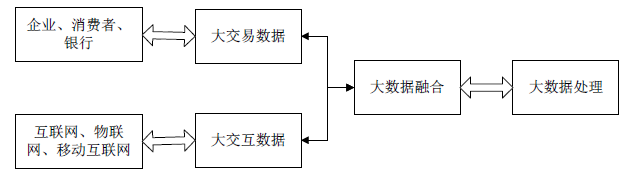
\includegraphics[width=\textwidth]{Figures/data.png}
\end{generalfig}

\subsection{表格}

如\autoref{tab:heightweight}所示
\begin{generaltab}{某校学生升高体重样本}{tab:heightweight}
    \begin{tabularx}{\textwidth}{lCCC}
        \toprule
        序号&年龄&身高&体重\\
        \midrule
        1&14&156&42\\
        2&16&158&45\\
        3&14&162&48\\
        4&15&163&50\\
        \cmidrule{2-4} %添加2-4列的中线
        平均&15&159.75&46.25\\
        \bottomrule
    \end{tabularx}
\end{generaltab}


\subsection{公式}
在文中引用公式可以这么写:$a^2+b^2=c^2$这是勾股定理,他还可以表示为$c=\sqrt{a^2+b^2}$,还可以让公式单独一段并且加上编号,如\autoref{eq:pingfanghe}所示
\begin{equation}
	\sin^2{\theta}+\cos^2{\theta}=1 
    \label{eq:pingfanghe}
\end{equation}


\subsection{列表}

计数列表
\begin{enumerate}
    \item 第一项
        \begin{enumerate}
            \item 第一项中的第一项
            \item 第一项中的第二项
        \end{enumerate}
    \item 第二项
    \item 第三项
\end{enumerate}

不计数列表
\begin{itemize}
    \item 第一项
    \begin{itemize}
        \item 第一项中的第一项
        \item 第一项中的第二项
    \end{itemize}
    \item 第二项
    \item 第三项
\end{itemize}


\section{结尾}
%生成参考文献
%使用方法:\bibliography{参考文件1文件名, 参考文献2文件名, ...}
\bibliography{Bibs/mybib}
%签名页
\signature
\end{document}
